\section{Towards Quantum Field Theory}

The concept of a \textbf{field} is central to modern physics, describing how physical quantities vary over space and time. It was introduced in the 19th century to explain phenomena such as electromagnetism and gravity, in order to move away from the idea of \textit{action at a distance}:
\begin{itemize}
  \item The \textbf{gravitational field}, described by Newton's law of universal gravitation, which explains the attraction between masses.
  \item The \textbf{electromagnetic field}, unified by Maxwell's equations, which describes electric and magnetic phenomena and their interactions with charged particles.
\end{itemize}
In this framework, particles interact locally through fields, rather than instantaneously over a distance.

Photons, the quanta of the electromagnetic field, mediate electromagnetic interactions; they represent the field's excitations around its ground state, thus allowing for the exchange of energy and momentum between charged particles. This description seems to elect the field as the fundamental entity, with particles being secondary manifestations. However, matter particles, such as electrons and quarks, seem to be more fundamental, as they constitute the building blocks of matter. This duality raises the question: which is more fundamental, fields or particles?\footnote{If we were to choose particles as fundamental, we would face the challenge of explaining how they interact at a distance, and fields like the EM one would be described as classical limits of a collection of photons.}

Quantum Field Theory provides a framework in which \textbf{fields are the fundamental quantities} and particles are viewed as excitations of underlying fields that permeate space and time, rather than as independent entities. Each type of particle corresponds to a specific field:
\begin{itemize}
    \item The \textbf{EM field} gives rise to photons, which mediate electromagnetic interactions.
    \item The \textbf{electron field} (Dirac) gives rise to electrons and positrons.
    \item The \textbf{quark fields} (Dirac) give rise to quarks, which combine to form protons and neutrons.
    \item The \textbf{Higgs field} (Klein-Gordon) is responsible for giving mass to particles through the Higgs mechanism.
\end{itemize}
Particles are thus seen as localized excitations or quanta of their respective fields around their ground states, and interactions between particles are understood as interactions between these fields.

\subsection*{Properties of the New Approach}

The new framework of QFT has several important properties, which are granted by the formulation itself:
\begin{enumerate}[label=(\roman*),align=left,itemsep=1.0\baselineskip]
  \item \textbf{Locality}:\\
  Interactions occur at specific points in space and time, ensuring that cause and effect are preserved.

  \item \textbf{Causality}:\\
  No information or influence can travel faster than the speed of light, preserving the causal structure of spacetime. \textit{Intuitively}, consider a spacetime event where a particle-antiparticle pair is created, moves apart, and later annihilates (space-like separated events which could be seen in opposite causal order by an external observer). One description is that the particle travels forward in time and annihilates with the antiparticle. An equivalent view is that the antiparticle represents a particle propagating backward in time. In quantum field theory, what matters are the probability amplitudes for such processes, and this reinterpretation ensures that they remain causal: all contributions respect the light cone structure, and no amplitude allows information to propagate faster than light.

  \item \textbf{Particle/antiparticle creation/annihilation}:\\
  The framework naturally incorporates processes where particles can be created or destroyed, since fields can describe systems with infinite degrees of freedom. Let us consider how coordinates describe a system in different contexts:
  \begin{itemize}
    \item \textbf{QM}: \((\mathbf{x},t) \to (\hat{\mathbf{x}}, \hat{t})\).\\
    The position and time of a particle are promoted to operators acting on a Hilbert space via \textit{canonical quantization}.\footnote{This process involves promoting classical fields to operator-valued distributions by imposing canonical commutation relations.} The number of particles is fixed, and creation/annihilation processes are not described.
    \item \textbf{QFT}: \((\mathbf{x},t) \to \phi(\mathbf{x},t) \to \hat{\phi}(\mathbf{x},t)\).\\
    The field configuration \(\phi(\mathbf{x},t)\) account for infinite degrees of freedom; it is promoted to an operator-valued distribution \(\hat{\phi}(\mathbf{x},t)\) acting on a Fock space, which can accommodate states with varying numbers of particles. Spacetime coordinates are interpreted as continuous labels for infinite field operators, not as operators themselves.
  \end{itemize}
  We can now describe processes such muon decay \(\mu^- \to e^- + \bar{\nu}_e + \nu_\mu\), where a muon transforms into an electron, an electron antineutrino, and a muon neutrino. This process involves annihilation and creation of particles, varying even the number of particles involved, which is naturally described in QFT.
    
  \item \textbf{Undistinguishability of particles of identical type}:\\
  Particles of the same type are fundamentally indistinguishable, even if they were created in different processes and in distant spacetime regions. \textit{Example}: protons produced in supernovae billions of light years away and in particle accelerators here on Earth are identical. This indistinguishability is naturally incorporated in QFT, where particles are excitations of the same underlying field which fills the entire universe.
    
  \item \textbf{Correct spin-statistics relations}:\\
  Undistinguishability for identical particles leads to the requirement that the quantum states of a system of multiple identical particles must be either symmetric (for bosons) or antisymmetric (for fermions) under the exchange of any two particles. This requirement is known as the \textbf{spin-statistics theorem}, which states that particles with integer spin (bosons) obey Bose-Einstein statistics, while particles with half-integer spin (fermions) obey Fermi-Dirac statistics:
  \begin{itemize}
    \item \(\psi\) is symmetric under exchange \(\psi(\dots\, x_i\, \dots\, x_j\, \dots) = \psi(\dots\, x_j\, \dots\, x_i\, \dots)\):\\
    Bosons (integer spin) can occupy the same quantum state, leading to phenomena like \textbf{Bose-Einstein condensation}.
    \item \(\psi\) is antisymmetric under exchange \(\psi(\dots\, x_i\, \dots\, x_j\, \dots) = -\psi(\dots\, x_j\, \dots\, x_i\, \dots)\):\\
    Fermions (half-integer spin) obey the \textbf{Pauli exclusion principle}, which prevents them from occupying the same quantum state.
  \end{itemize}
  In QM this relations are imposed as an additional postulate, while in QFT it emerges naturally from the commutation relations of field operators. While quantizing a field, one has to define strictly spin-statistics relations, imposing commutation relations for bosonic fields and anticommutation relations for fermionic fields:
  \[
    \begin{aligned}
      &\text{Bosons:} \quad [\hat{\phi}(\mathbf{x},t), \hat{\phi}(\mathbf{y},t)] = 0, \quad [\hat{\phi}(\mathbf{x},t), \hat{\pi}(\mathbf{y},t)] = i\delta^3(\mathbf{x}-\mathbf{y}),\\
      &\text{Fermions:} \quad \{\hat{\psi}_\alpha(\mathbf{x},t), \hat{\psi}_\beta(\mathbf{y},t)\} = 0, \quad \{\hat{\psi}_\alpha(\mathbf{x},t), \hat{\psi}^\dagger_\beta(\mathbf{y},t)\} = \delta_{\alpha\beta} \delta^3(\mathbf{x}-\mathbf{y}).
    \end{aligned}
  \]
  This ensures \textbf{consistency}: \(E>0\) and no negative norm states for every particle; the correct statistics for particles emerge naturally from the field quantization process and the underlying symmetries of the theory.
\end{enumerate}

Quantum Field Theory provides a consistent and comprehensive description of the fundamental particles and their interactions, not only in relativistic regimes but also in non-relativistic ones with variable number of particles. It has been remarkably successful in explaining a wide range of phenomena at the fundamental level, from the behavior of condensed matter systems to high energy particle collisions, from quantum gravity to cosmology. It also contributed to pure mathematical developments, in fields such as topology and geometry.

\subsection*{Units and Scales}

In nature we have three fundamental dimensionfull constants:
\begin{itemize}
  \item The speed of light in vacuum \(c\), which relates space and time.
  \item The reduced Planck constant \(\hbar\), which relates energy and frequency.
  \item The gravitational constant \(G\), which sets the strength of gravitational interactions.
\end{itemize}
Let us analyze their dimensions in terms of mass \(M\), length \(L\), and time \(T\):
\[
  \begin{aligned}
    [c] &= \frac{L}{T},\\
    [\hbar] &= [E] T = \frac{M L^2}{T},\\
    [G] &= \frac{[E] L}{M^2} = \frac{L^3}{M T^2}.
  \end{aligned}
\]
From these three constants we can construct a system of \textbf{natural units}, by setting \(c = \hbar = 1\). This choice simplifies equations and calculations in theoretical physics, particularly in QFT and quantum gravity. In this system, all physical quantities can be expressed in terms of a single unit, typically mass (or energy), and even length and time have the same dimension \(L=T\).
For the \textbf{Compton wavelength} in natural units we have:\footnote{The Compton wavelength \(\lambda_c\) of a particle with mass \(m\) is given by \(\lambda_c = \frac{\hbar}{mc}\). It represents a fundamental limit to the precision with which we can localize a particle, as attempting to confine it to a region smaller than its Compton wavelength would require energies sufficient to create particle-antiparticle pairs, thus undermining the notion of a single, localized particle.}
\[
  \lambda_c = \frac{\hbar}{mc} = \frac{1}{m} \implies L = \frac{1}{M}.
\]
Thus since \(L = T = \frac{1}{[E]} = \frac{1}{M}\), we can express the dimensions of the three constants as:
\[
  [c] = 1, \quad [\hbar] = 1, \quad [G] = \frac{L}{M} = \frac{1}{M^2},
\]
The gravitational constant \(G\) has dimensions of inverse mass squared, indicating that gravitational interactions become significant at very high energy scales.

Sometimes \textit{mass dimensions} will come in handy, especially when dealing with fields and coupling constants. They consists in the dimensions of a quantity expressed in terms of mass only. For example, in natural units:
\[
  [c] = [\hbar] = 0, \quad [G] = -2,\quad [E] = 1.
\]

The \textbf{Planck scale} is the energy scale at which quantum effects of gravity become significant, and it is defined using the three fundamental constants:
\[
  M_P = \sqrt{\frac{\hbar c}{G}} \approx \SI{1.22e19}{\giga\electronvolt}.
\]
It represents the scale where our current understanding of physics, based on QFT and General Relativity, breaks down, and a theory of quantum gravity is required. It is related to the \textbf{Planck length}:
\[
  l_P = \sqrt{\frac{\hbar G}{c^3}} \approx \SI{1.62e-35}{\meter}.
\]

In the following figure we summarize the energy scales of fundamental physics, from the Planck scale to the Hubble scale.
\begin{figure}[H]
\centering
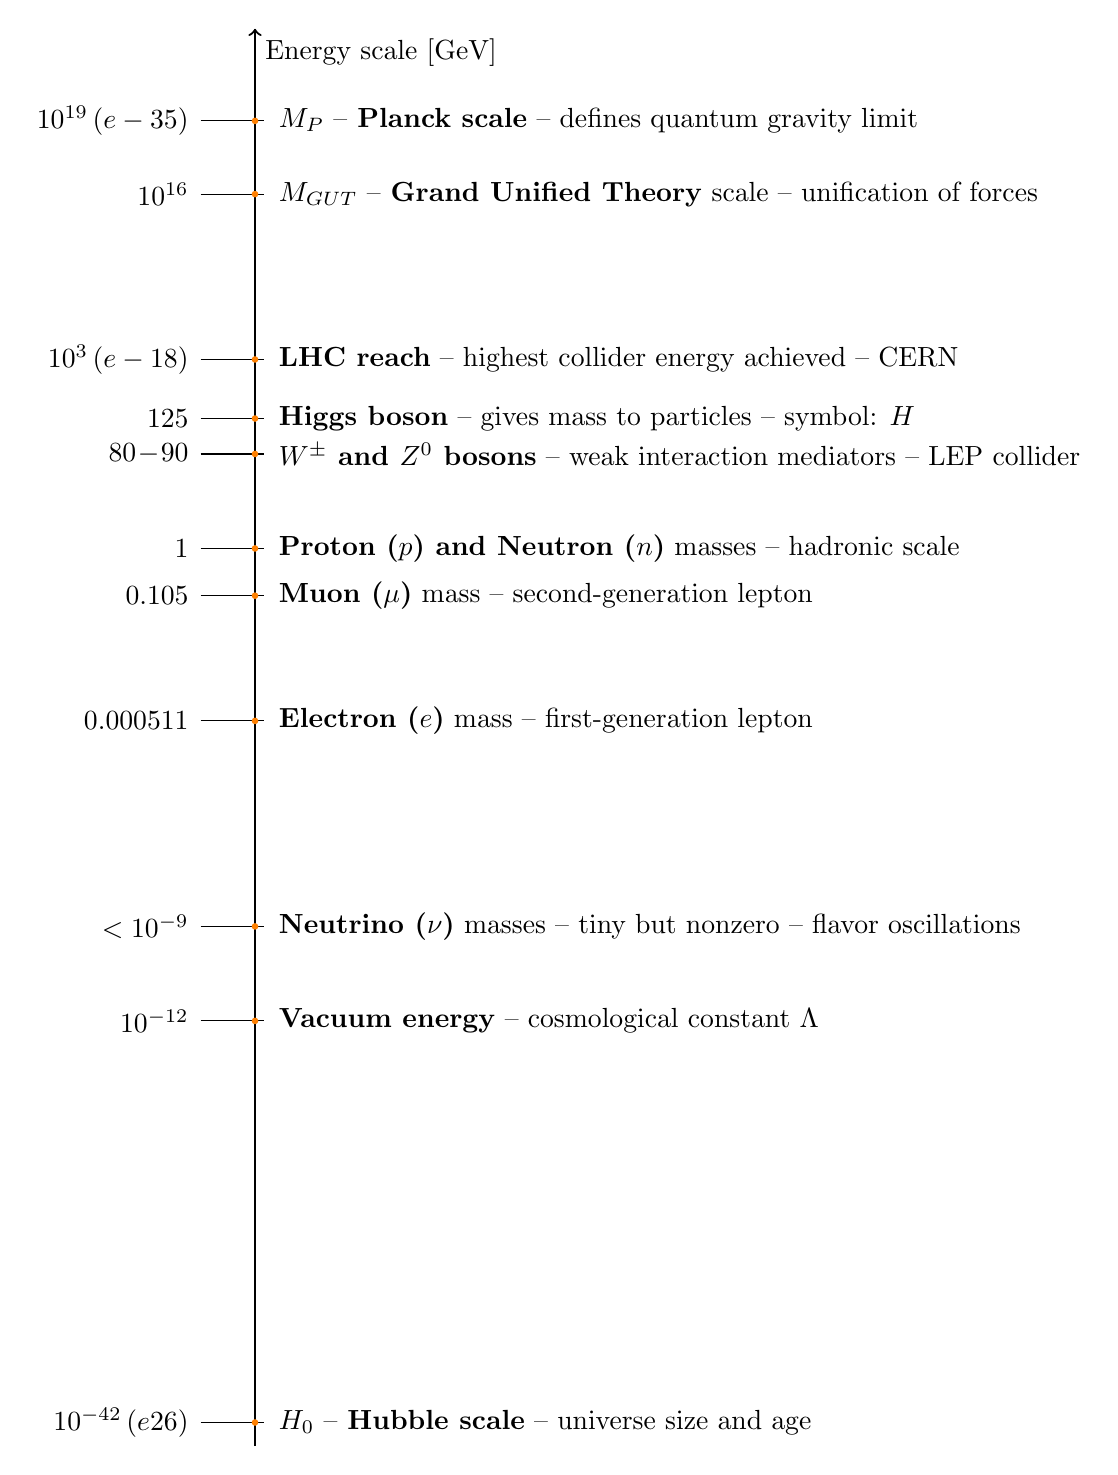
\begin{tikzpicture}[scale = .6]

  \draw[thick,->] (0,0) -- (0,30) node[anchor=north west]{Energy scale [GeV]};

  \foreach \y/\E/\desc in {
    16.1/{$10^{19} \, (\SI{e-35}{\meter})$}/ $M_P$ -- \textbf{Planck scale} -- defines quantum gravity limit,
    13/{$10^{16}$}/$M_{\text{GUT}}$ -- \textbf{Grand Unified Theory} scale -- unification of forces,
    6/{$10^3 \, (\SI{e-18}{\meter})$}/\textbf{LHC reach} -- highest collider energy achieved -- CERN,
    3.5/{$125$}/\textbf{Higgs boson} -- gives mass to particles -- symbol: $H$,
    2/{$80\!-\!90$}/\textbf{$W^\pm$ and $Z^0$ bosons} -- weak interaction mediators -- LEP collider,
    -2/{$1$}/\textbf{Proton ($p$) and Neutron ($n$)} masses -- hadronic scale,
    -4/{$0.105$}/\textbf{Muon ($\mu$)} mass -- second-generation lepton,
    -9.3/{$0.000511$}/\textbf{Electron ($e$)} mass -- first-generation lepton,
    -18/{$<10^{-9}$}/\textbf{Neutrino ($\nu$)} masses -- tiny but nonzero -- flavor oscillations,
    -22/{$10^{-12}$}/\textbf{Vacuum energy} -- cosmological constant $\Lambda$,
    -39/{$10^{-42} \, (\SI{e26}{\meter})$}/$H_0$ -- \textbf{Hubble scale} -- universe size and age
  }{
    \pgfmathsetmacro{\yy}{(\y + 40) * 0.5}
    \draw (-1.15,\yy) -- (0.2,\yy);
    \fill[orange] (0,\yy) circle (2pt);
    \node[anchor=east] at (-1.2,\yy) {\E};
    \node[anchor=west,align=justify] at (0.3,\yy) {\desc};
  }

\end{tikzpicture}
\end{figure}

\section{Mechanical Model of a Quantum Field}